\documentclass[UTF8]{ctexart} %使用ctex包,中文支持
\usepackage{amsmath}  %数学公式
\usepackage{graphicx} %插图
\usepackage{fancyhdr} %个性化页眉页脚
\usepackage{geometry} %页边距
\usepackage{bm}  % 公式加粗
\usepackage{float} %为了在分栏下插入图片
\usepackage{ulem}  % 换行下划线
%\usepackage{setspace} %行间距
\usepackage{multicol} %用于实现在同一页中实现不同的分栏
\geometry{a4paper,left=2cm,right=2cm,top=2cm,bottom=2cm} % 页边距设置

\title{信息论笔记}
\author{宋佳欢}
\pagestyle{plain}

\begin{document}
	\maketitle
	\tableofcontents
	\songti \zihao{-4}
	
	\section{信息熵}
		信息量$I(x)=f\big(p(x)\big)$,函数$f$需满足下列四个条件:
		
		\quad1.$f$单调递减,事件发生的概率越小,获得的信息量越大。
		
		\quad2.当$p(x)=1$,$f\big(p(x)\big)=0$
		
		\quad3.当$p(x)=0$,$f\big(p(x)\big)=\infty$
		
		\quad4.两件独立事件同时发生的获取的信息之和为$I(x,y)=I(x)+I(y)=f\big(p(x)\big)+f\big(p(y)\big)=f\big(p(x,y)\big)$
		
		因此,$p(x,y)=p(x)p(y)$。根据这个关系,$I(x)$与$p(x)$一定为对数关系。
		
		根据上述四个条件可得:\[I(x)=-logp(x)\]
		其中负号是用来保证信息量是正数或者零。而$log$函数基的选择是任意的(信息论中基常常选择为2,因此信息的单位为比特bits,即信息需要的编码长度;而机器学习中基常常选择为自然常数,因此单位常常被称为奈特nats;底数为10,单位则为Hart)。
		
		$I(x)$也被称为随机变量x的自信息 (self-information),\uline{描述的是随机变量的某个事件发生所带来的信息量}。
		
		现在假设一个发送者想传送一个随机变量的值给接收者。那么在这个过程中,他们传输的平均信息量可以通过求$I(x)$关于概率分布$p(x)$的期望求得,随机变量X的\uline{信息熵}的定义:
		\[H(X)= -\sum_{i=1}^np(x_i)logp(x_i)\]
		熵越大,随机变量的不确定性就越大。是对所有可能发生的事件产生的信息量的期望。
		
		\subsection{代数性质}
			\subsubsection{对称性}
				变量$p_1,p_2,\cdots,p_r$的顺序任意互换,熵不变。
				\[H(p_1,p_2,\cdots,p_r) = H(p_2,\cdots,p_r,p_1) = H(p_r,p_1,p_2,\cdots,p_{r-1})\]
			\subsubsection{非负性}
				\[H(p_1,p_2,\cdots,p_r) \geq 0\]
			\subsubsection{连续性}
				$H(p_1,p_2,\cdots,p_r)$ 是$p_i$的连续函数。
			\subsubsection{扩展性}
				\[\lim_{\varepsilon\rightarrow0}H(p_1,p_2,\cdots,p_i-\varepsilon,\cdots,p_r,\varepsilon_1,\varepsilon_2,\cdots,\varepsilon_k)=H(p_1,p_2,\cdots,p_r)\]
				其中每个$\varepsilon$都趋于0。当信源的消息集中的消息数增多时,因为这些消息对于的概率很小(比重很小),所以信源的熵不变。
			\subsubsection{可加性}
				统计独立的两个信源X,Y的两个联合信源的熵等于分别熵之和:
				\[H(X,Y) = H(X)+H(Y)\]	
				\[\begin{aligned}
					H(X,Y)&=-\sum_{i=1}^n\sum_{j=1}^mp_iq_jlogp_iq_j\\
					& =-\sum_{i=1}^n\sum_{j=1}^mp_iq_jlogp_i-\sum_{i=1}^n\sum_{j=1}^mp_iq_jlogq_j\\
					& =-\sum_{i=1}^n\big(\sum_{j=1}^mp_iq_j\big)logp_i-\sum_{j=1}^m\big(\sum_{i=1}^np_iq_j\big)logq_j\\
					& =-\sum_{i=1}^np_ilogp_i-\sum_{j=1}^mq_jlogq_j = H(X)+H(Y)
				\end{aligned}\]
			\subsubsection{递增性}
				将信源X中的其中一个元素划分成m个元素,这m个元素的概率之和等于原元素的概率,熵增加。
				\[H_{n+m-1}(p_1,p_2,\cdots,p_{n-1},q_1,q_2,\cdots,q_m) = H_n((p_1,p_2,\cdots,p_{n-1},p_n)
				+p_nH_m(\frac{q_1}{p_n},\frac{q_2}{p_n},\cdots,\frac{q_m}{p_n})\]
		\subsection{解析性质}
			\subsubsection{最大离散熵定理}
				在离散信源情况下,信源各符号等概率分布时,熵达到最大。(概率分布越接近平均分布,熵越大)
				\[H(p_1,p_2,\cdots, p_r) \leq H(\frac{1}{r},\frac{1}{r},\cdots,\frac{1}{r})\leq logr\]
			\subsubsection{上凸性}
				熵函数是严格的上凸函数:
				\[H(\theta P_1+(1-\theta) P_2) > \theta H( P_1)+(1-\theta)H(P_2)\]
	\section{信道}
		离散单符号信道可用传递概率表示:
			\[ 
			\begin{bmatrix} 
			P(b_1|a_1) &  P(b_2|a_1) & \cdots & P(b_s|a_1)\\
			P(b_1|a_2) &  P(b_2|a_2) & \cdots & P(b_s|a_2)\\
			\vdots & \vdots &   & \vdots\\
			(b_1|a_r) &  P(b_2|a_r) & \cdots & P(b_s|a_r)
			\end{bmatrix} 
			 \]
			 a为输入,b为输出。且传递矩阵(信道矩阵)每一行的元素相加等于1,即:
			 \[\sum_{j=1}^sP(b_j|a_i)=1\]
			 $P(b_i|a_i)$表示发送a收到b的概率(前向概率)描述了信道噪声的特征,$P(a_i|b_i)$表示接受到了$b_i$,发送端发送$a_i$的概率(后向概率)。
		\subsection{互信息与平均互信息}
			互信息(Mutual Information):$I(a_i;b_j)$表示接受到$b_j$后,能从$b_j$获得的关于$a_i$的信息量。
			\uline{互信息的三种写法:}
			\[\begin{aligned}
				I(a_i;b_j) &= I(a_i) - I(a_i | b_j)\\
				& =I(b_j) - I(b_j | a_i)\\
				&  = I(a_i) + I(b_j) -I(a_i,b_j)
			\end{aligned}\]
			
			但是单个样本的互信息不足以表示整个系统,因此需要对多个样本取期望,即平均互信息:
			\[I(X;Y) = E_{P(X,Y)}\{I(a_i;b_j)\}\]
			
			对于单个样本的互信息,其值可正可负或为零,但是平均互信息一定不会为负值。
			
			证明:
			\[I(X;Y) = E_{P(X,Y)}\{I(a_i;b_j)\} = \sum_i\sum_j P(a_i,b_j)log\frac{P(a_i,b_j)}{P(a_i)P(b_j)}\]
			\[-I(X;Y) = \sum_i\sum_j P(a_i,b_j)log\frac{P(a_i)P(b_j)}{P(a_i,b_j)}\]
			根据琴生不等式,以及:
			\[\sum_i\sum_jP(a_i)P(b_j)=1\]
			所以
			 \[-I(X;Y) = \sum_i\sum_j P(a_i,b_j)log\frac{P(a_i)P(b_j)}{P(a_i,b_j)} \leq log\Big(\sum_i\sum_j P(a_i,b_j)\frac{P(a_i)P(b_j)}{P(a_i,b_j)}\Big)=log1=0\]
			 即
			 \[I(X;Y) \geq0\]
			 
			 \uline{互信息有三种写法,平均互信息也衍生出三种写法:}
				\[\begin{aligned}
				I(X;Y) &= H(X) - \underbrace{H(X|Y)}_{\text{疑义度(损失熵)}}\\
				& =H(Y)-\underbrace{H(Y|X)}_{\text{噪声熵}}\\
				&  =H(X)+H(Y)-\underbrace{H(XY)}_{\text{联合熵(共熵)}}
				\end{aligned}\]
		\subsection{信道容量}	
			每一个信道都有一个最大的信息传输率,这个最大传输率定义为:
			\[C = \max_{P(x)}\{I(X;Y)\}\quad \text{单位:比特/符号}\]
			
			信道单位时间内平均传输的最大信息量为:
			\[C_t = \frac{C}{t}\quad \text{单位:比特/秒}\]
			
		\subsubsection{无噪无损信道(输入输出一一对应)}
			该信道的信道矩阵每行每列仅有一个1,其他都为0。
			
			这类信道的平均互信息为:
			 \[\begin{aligned}
			 I(X;Y) &= H(X) - \underbrace{H(X|Y)}_{\text{疑义度=0}}\\
			 & =H(Y)-\underbrace{H(Y|X)}_{\text{噪声熵=0}}\\
			 &  =H(X) = H(Y)
			 \end{aligned}\]
			 当输入信源确定后,接收到的符号也确定,为确定性事件,所以噪声熵为0;同理疑义度(损失熵)也为0。
			 
			 当输入信源等概率分布时,此类信道的信息传输率达到极大值:
			 \[C = \max_{P(x)}\{I(X;Y) = \max_{P(x)}H(X) = logr\]
		\subsubsection{无损信道}	
			一个输入对应多个输出,但是每个输出只对应一个输入。
			\begin{figure}[H]
				\centering{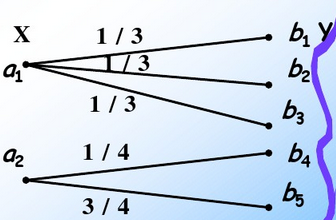
\includegraphics[scale=0.4]{1.png}}
			\end{figure}
			
			\textbf{信道矩阵特点:}信道矩阵中每列有且仅有一个非零元素。
			
			这类信道的损失熵(疑义度)=0,即当输出符号确定后,输入符号也随之确定。噪声熵不为0。
			
			平均互信息为:
			\[I(X;Y) = H(X)<H(Y)\]
			
			信道容量为(信源等概率分布时取到):
			\[C = \max_{P(x)}H(X) = logr\]
		\subsubsection{无噪有损信道}
			多个输入对应一个输出,一个输出对应多个输入。
			\begin{figure}[H]
				\centering{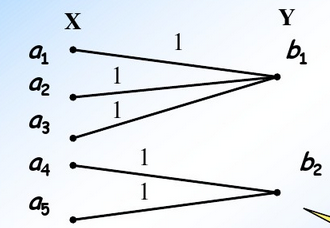
\includegraphics[scale=0.4]{2.png}}
			\end{figure}
			\textbf{信道矩阵特点:}每行仅有一个非零元素。
			
			这类信道的噪声熵为0,损失熵(疑义度)不为0。
			
			平均互信息:
			\[I(X;Y) = H(Y)<H(X)\]
			
			信道容量为(总能找到一个最佳的输入分布X,使得输出Y达到等概率分布):
			\[C = \max_{P(x)}H(Y) = logr\]
		\subsubsection{对称离散信道}
			\textbf{信道矩阵特点:}信道矩阵中的每一行都是由同一$\{p_1^,,p_2^,,...,p_s^,\}$集的各个元素不同排列组成。每一行都是由同一$\{q_1^,,q_2^,,...,q_r^,\}$集的各个元素不同排列组成。
			平均互信息:
			\[I(X;Y) = H(Y)-H(Y|X)\]
			\[H(Y|X) = \sum_XP(x)|sum_YP(y|x)log\frac{1}{P(y|x)} = \sum_XP(x)H(Y|X=x)\]
			x取某一值时,$H(Y|X=x)$即为对信道矩阵的某一行求和,因为信道矩阵每一行都是相同元素的排列组合,所以该值对于所以的x都相同,即与x无关:
			\[H(Y|X=x) = H(p_1^,,p_2^,,...,p_s^,)\]
			
			所以信道容量C为:
			\[C = \max_{P(x)}[H(Y) -  H(p_1^,,p_2^,,...,p_s^,)]\]
			问题转化为求一个输入分布$P(x)$,使得$H(Y)$取最大值的问题。若输出信号Y等概率分布,就能得到最大的$H(Y)=logs$。
			
			每个输出符号的概率为:
			\[P(y_i) = \sum_{X}P(x)P(y_i|x)\]
			
			将输入信号设为等概率分布,即$P(x)=\frac{1}{r}$,上式变为:
			\[P(y_i) = \sum_{X}\frac{1}{r}P(y_i|x) = \frac{1}{r}\sum_{X}P(y_i|x)\]
			
			由于信道矩阵的每一列都是相同元素的不同组合,所以$\sum_{X}P(y_i|x)$不变,为信道矩阵每一列的和$\sum_{i=1}^sq_i^,$。即当输入信号等概率时,输出信号也等概率。
			
			对称离散信道的信道容量为:
			\[C =  logr -  H(p_1^,,p_2^,,...,p_s^,),(\text{比特/符号})\]
		\subsubsection{准对称信道}
			\textbf{信道矩阵特点:}1.行可排。2.列不可排,若分为若干子集,在子集中可排。
			
			将信道矩阵按列分为m个子集,每个子集含有$s_l$列,$l=1,2,...,m$。$P(b_l)$为第$l$个子集输出符号的平均概率。
			
			准对称信道的信道容量为:
			\[C = -\sum_{l=1}^ms_lP(b_l)log(b_l) -H(p_1^,,p_2^,,...,p_s^,) \]
			
		\subsubsection{一般离散信道(等量平衡定理)}
			求信道容量,等价于一个带约束的优化问题:
			\[C = \max_{P(x)}I(X;y),\quad s.t.\sum_{i=1}^rP(a_i)=1\]
			
			利用拉格朗日乘子法,做辅助函数:
			\[F(p(a_1),p(a_2),...p(a_r),\lambda) = I(X;Y)- \lambda\bigg[\sum_{i=1}^rP(a_i)-1\bigg]\]
			分别对$p(a_1),p(a_2),...p(a_r)$求偏导,并置之为零。
			
			\[\begin{aligned}
			\frac{\partial F}{\partial P(a_i)} &= \frac{\partial I(X;Y)}{\partial P(a_i)}-\lambda\\
			&=\sum_{j=1}^sp(b_j|a_i)ln\frac{p(b_j|a_i)}{p(b_j)}-1-\lambda\\
			&=I(a_i;Y)-1-\lambda
			\end{aligned}\]
			
			即:
			\[\sum_{j=1}^sp(b_j|a_i)ln\frac{p(b_j|a_i)}{p(b_j)}= 1+\lambda\]
			假设使$I(X;Y)$达到最大值的输入信源的概率是${p_1,p_2,...p_r}$,两边关于输入信源的概率求积分(求和):
			\[\sum_{i=1}^r\sum_{j=1}^sp_ip(b_j|a_i)ln\frac{p(b_j|a_i)}{p(b_j)}= \sum_{i=1}^rp_i(1+\lambda)\]
			等式左边就是信道容量,所以:
			\[C = 1+\lambda\]
			\textbf{等量平衡定理}:当信道的平均互信息达到信道容量时,输入信源符号集中的每个信源符号x对输入端提供的互信息都相等,除概率为0的符号以外。
			
		\subsubsection{可逆矩阵信道的信道容量}
			略(手写笔记)
		\subsubsection{信道容量的迭代计算}	
			一般信道容量计算复杂,使用迭代的方法对信道容量近似计算。
				
			信道的平均互信息是先验概率$p(a_i)$和后验概率$p(a_i|b_j)$的一个函数:
			\[I(X;Y) = H(X)-H(X|Y) = -\sum_{i=1}^rp(a_i)lnp(a_i)+\sum_{i=1}^r\sum_{j=1}^sp(a_i)p(b_j|a_i)lnp(a_i|b_j)\]
			而这两个变量之间并不是独立的,满足:
			\[p(a_i|b_j) = \frac{p(a_i)p(b_j|a_i)}{\sum_{i=1}^rp(a_i)p(b_j|a_i)}\]
			
			1.固定$p(a_i)$,求解使得$I(X;Y)$最大的$p(a_i|b_j)$。
			
			2.固定$p(a_i|b_j)$,求解使得$I(X;Y)$最大的$p(a_i)$。
			
			3.重复上述步骤,不断迭代至收敛。
	\subsection{平均互信息量的不增性}
		略(手写笔记)
		
	\section{多符号离散信源与信道}
		\subsection{多符号信源基本概念}
			信源在每一个单位时间内,以一定的概率$P(a_{il})(l=1,2,3,...)$,发出信源符号集$X:\{a_1,a_2,\cdots,a_r\}$中的某一符号$a_{il}(l=1,2,3,...)\subset\{a_1,a_2,\cdots,a_r\}$,随着时间推移,形成无限长的随机符号序列$(a_{i1},a_{i2},\cdots)$,相当与无限长的随机变量序列$(X_1X_2\cdots X_N\cdots)$
		\subsection{离散平稳信源的定义}
			多符号离散信源$\bm{X} = X_1X_2\cdots X_N\cdots$的各维联合概率分布,不随时间发生变化,与其实时刻的选择无关。若Q和T表示两个任意的时刻,则有:
			\[P\{X_Q=a_i\} = P\{X_T=a_i\} =p(a_i)\]
			\[P\{X_Q=a_i,X_{Q+1}=a_j\} = P\{X_T=a_i,X_{T+1}=a_j\} =p(a_i,a_j)\]
			\[\cdots\]
			\[\text{条件概率形如:}P\{X_{Q+1}=a_j|X_Q=a_i\} = P\{X_{T+1}=a_j|X_T=a_i\} =p(a_j|a_i)\]
			\subsubsection{数学模型}
				将随机变量序列,将每N个变量分为一组,假定组与组之间统计独立,组内的N个信源符号仍然保持统计依赖关系。 在定长N和统计独立的假设下,长度为N的随机变量序列
				\[\bm{X} = X_1X_2\cdots X_N\]
				\[\text{每一组消息:}\alpha_i = (a_{i1}a_{i2}\cdots a_{iN})\]
				\[\sum_{i=1}^{r^N}p(\alpha_i) = 1\]
		\subsection{离散平稳无记忆信源的信息熵}
			离散平稳无记忆信源X的N次扩展信源$X_N$的概率:
			\[P(X_N) = P(X_1X_2\cdots X_N) = P(X_1)P(X_2)\cdots P(X_N)\]
			
			某一消息的概率:
			\[p(\alpha_i) = p(\alpha_{i1}\alpha_{i2}\cdots\alpha_{iN}) = p(\alpha_{i1})p(\alpha_{i2})\cdots p(\alpha_{iN}\]
			
			\textbf{定理:(证明P194)}
			\[ H(X_N) =H(X_1X_2\cdots X_N) = NH(X) \]
		\subsection{离散平稳有记忆信源的信息熵}
			离散平稳无记忆信源X的N次扩展信源$X_N$的概率:
			\[P(\bm{X}) = P(X_1X_2\cdots X_N) = P(X_1)P(X_2|X_1)P(X_3|X_1X_2)\cdots P(X_N|X_1X_2\cdots X_{N-1})\]
			
			某一消息的概率:
			\[p(\alpha_i) = p(\alpha_{i1}\alpha_{i2}\cdots\alpha_{iN}) = p(\alpha_{i1})p(\alpha_{i2}|\alpha_{i1})p(\alpha_{i3}|\alpha_{i1}\alpha_{i2})\cdots p(\alpha_{iN}\alpha_{i1}\alpha_{i2}\cdots\alpha_{iN-1})\]
			
			\textbf{定理:(证明P201)}
			\[ H(\bm{X}) =H(X_1X_2\cdots X_N) =H(X_1)+H(X_2|X_1)+H(X_3|X_1X_2)+\cdots+H(X_N|X_1X_2\cdot X_{N-1})\]
			
			\textbf{定理:(证明P203)}
			\[H(X_k|X_1X_2\cdots X_{k-1}) \leq H(X_k)\]
		
			\textbf{定理:(证明P205)}
			\[H(X_k|X_1X_2\cdots X_{k-1}) \leq H(X_{k-1}|X_1X_2\cdots X_{k-2})\]
			
			\textbf{推论:(证明P206)}
			\[logr \geq H(X_1) \geq H(X_2|X_1) \geq H(X_3|X_1X_2)\geq\cdots\geq H(X_N|X_1X_2\cdots X_{N-1})\]
			
			
		\subsection{离散平稳有记忆信源的极限熵}
			定义:离散平稳有记忆信源X的N次扩展信源$\bm{X} = X_1X_2\cdots X_N$的平均符号熵(每发出一个符号提供的平均信息量):
			\[H_N(\bm{X}) = H_N(X_1X_2\cdots X_N) = \frac{ H(X_1X_2\cdots X_N)}{N}\]
			
			极限熵(信源处于稳定状态时,每发出一个符号提供的平均信息量):
			\[H_\infty = \lim_{N\rightarrow\infty}H_N(\bm{X}) =\lim_{N\rightarrow\infty} \frac{ H(X_1X_2\cdots X_N)}{N}\]
			去除了“消息定长”和“消息与消息之间统计独立”的两个人为假设。
			
			\textbf{定理:(证明P210)}
			\[H_\infty = \lim_{N\rightarrow\infty}H(X_N|X_1X_2\cdots X_N)\]
		\subsection{Markov信源的极限熵}	
			信源X,任何时刻$t_{m+1}$随机变量$X_{m+1}$发出符号$a_{im+1}$只与前m个符号$(a_{i1},a_{i2},\cdots,a_{im})$有关,则称该离散平稳有记忆信源为m阶Markov信源。
			
			\textbf{定理:m-M信源消息的n步转移矩阵,等于一步转移概率矩阵的n次乘积(P215)}
			\[[P(n)] = [P]\cdot[P]\cdots[P]\]
			
			\textbf{定理:消息的极限概率$p(S_i)$是下列方程的唯一解(P217)}
			\[p(S_j) = \sum_{i=1}^{r^m}p(S_i)p(S_j|S_i)\]
			
			\textbf{定理:m-M信源的极限熵等于m阶条件熵(P225)}
			\[H_{\infty} = H(X_{m+1}|X_1X_2\cdots X_m) = -\sum_{i1=1}^{r^m}\sum_{j=1}^{r^m}p(S_i)p(S_j|S_i)logp(S_j|S_i)\]
			
		\subsection{信源的剩余度(冗余度)与结构信息}
			结构信息:
			\[I_{0\infty m} = \underbrace{H_0}_{logr}-H_{\infty m}\]
			$H_0$:信源能提供信息的最大能力,$H_{\infty m}$:信源X每个符号含有的平均信息量。
			
			剩余度(冗余度):
			\[\xi = \frac{I_{0\infty m}}{H_0} = 1-\frac{H_{\infty m}}{H_0}\]
			例如把“北京大学”压缩成“北大”,剩余度就减小了。但是剩余度大的消息的抗干扰能力越大。
			
		\subsection{无记忆扩展信道}
			性质:
			\[P(\bm{Y}|\bm{X}) = P(Y_1Y_2\cdots Y_N|X_1X_2\cdots X_N) = \prod_{k=1}^NP(Y_k|X_k)\]	
			
			\textbf{定理:}
			\[P(Y_K|X_1X_2\cdots X_k,Y_1Y_2\cdots Y_{k-1} )=P(Y_k|X_k)\quad\text{无记忆性}\]
			\[P(Y_1Y_2\cdots Y_{k-1} |X_1X_2\cdots X_k)=P(Y_1Y_2\cdots Y_{k-1} |X_1X_2\cdots X_{k-1})\quad\text{无预感性}\]
			
		\subsection{扩展信道的平均交互信息量}
			\[I(\bm{X;Y}) = \sum_{i=1}^{r^N}\sum_{j=1}^{s^N}p(\alpha_i\beta_j)log\frac{p(\beta_j|\alpha_i)}{p(\beta_j)}\]
			
			\textbf{定理:离散无记忆信道的N次扩展的平均交互信息量$I(\bm{X;Y})$,小于或等于信源X各个时刻通过无记忆信道的平均交互信息量之和}
				\[I(\bm{X;Y})\leq\sum_{k=1}^{N}I(X_k;Y_k)\]
			当且仅当信源时离散无记忆信源的N次扩展信源,等号成立。
		\subsection{无记忆扩展信道的信道容量}	
			\[\max(I(\bm{X;Y}))=\sum_{k=1}^{N}I(X_k;Y_k)=NC_0\]
			
		\subsection{独立并列信道的信道容量}	
			\textbf{定理:}
			\[I(\bm{X;Y}) = I(X_1X_2\cdots X_N|Y_1Y_2\cdots Y_N)\leq\sum_{k=1}^{N}I(X_k;Y_k)\]
			
			\textbf{定理:由N个信道构成的独立并列信道的联合信道容量$C_{N0}$,等于各信道自身的信道容量$C_k$之和}
			\[C_{N0} = \sum_{k=1}^NC_k\]
		
\end{document}